%\documentclass[a4paper,10pt,twoside]{article}
\documentclass[10pt,a4paper,twoside]{llncs}
\usepackage[left=3cm,right=3cm,top=2.5cm,bottom=2.5cm]{geometry}
%\usepackage[utf8x]{inputenc}
\usepackage[T1]{fontenc}
\usepackage[latin1]{inputenc}
\usepackage{amsmath,amsfonts,amssymb}%\usepackage{amsmath,amsfonts,amsthm,amssymb}
\usepackage{graphicx}
\usepackage{pstricks}    %for embedding pspicture.
\usepackage{epsfig}
\usepackage{algorithmic,algorithm}
%\usepackage{tikz}
%\usetikzlibrary{matrix}

\pagestyle{headings}%page numbers

%%%%%%%%%%%%%%%%%%%%%%%%%%% VERSIONES %%%%%%%%%%%%%%%%%%%%%%%%%%%%%%%%%%%
\usepackage{gitinfo}
\newcommand{\version}{github.Papers: \gitCommitterDate\;(revision \gitAbbrevHash) }
\newcommand{\todo}[1]{\texttt{\color{red}TODO:} ``\emph{#1}''}
\newcommand{\fixme}[1]{\texttt{\color{red}FIXME:} ``\emph{#1}''}
%%%%%%%%%%%%%%%%%%%%%%%%%%%%%%%%%%%%%%%%%%%%%%%%%%%%%%%%%%%%%%%%%%%%%%%%%
\newcommand{\tango}{\textsc{Tango}}
\newcommand{\sardana}{\textsc{Sardana}}
\newcommand{\taurus}{\textsc{Taurus}}
\newcommand{\atk}{\textsc{Atk}}
\newcommand{\zmq}{\textsc{$\varnothing$mq}}
\newcommand{\corba}{\textsc{Corba}}

%opening
\title{Ensuring \tango Control System}
\author{Sergi Blanch-Torn\'e\inst{1}, Ramiro Moreno Chiral\inst{2}}
 \institute{
 Escola Polit\`ecnica Superior, Universitat de Lleida. Spain.\\
 \email{\tt sblanch@alumnes.udl.es}
 \and 
 Departament de Matem\`atica. Universitat de Lleida. Spain.\\
 \email{\tt ramiro@matematica.udl.es}
 }

%%% Definiciones matem\'aticas especiales

\newcommand{\Z}{\ensuremath{\mathbb{Z}}}%                       Enteros
\newcommand{\Q}{\ensuremath{\mathbb{Q}}}%                       Racionales
\newcommand{\A}{\ensuremath{\mathcal{A}_{2}}}%                   Plano Af\'{\i}n
\newcommand{\Proy}{\ensuremath{\mathcal{P}_{2}}}%                Plano Proyectivo
\newcommand{\Jacob}{\ensuremath{\mathcal{J}_{2}}}%               Plano Jacobiano
\newcommand{\K}{\ensuremath{\mathbb{K}}}%                       Cuerpo en general
\newcommand{\F}{\ensuremath{\mathbb{F}}}%                       Cuerpo finito en general
\newcommand{\Fp}{\ensuremath{\mathbb{F}_p}}%                    Cuerpo finito de orden p (primo)
\newcommand{\EFp}{\ensuremath{E(\mathbb{F}_p)}}%                Curva el\'\{i}ptica sobre un cuerpo finito de orden p (primo)
\newcommand{\EFq}{\ensuremath{E(\mathbb{F}_q)}}%                Curva el\'\{i}ptica sobre un cuerpo finito
\newcommand{\Fm}{\ensuremath{\mathbb{F}_{2^m}}}%                Cuerpo finito de caractar\'{\i}stica 2, grado m
\newcommand{\EFm}{\ensuremath{E(\mathbb{F}_p)}}%                Curva el\'\{i}ptica sobre un cuerpo finito de caractar\'{\i}stica 2, grado m
\newcommand{\Fq}{\ensuremath{\mathbb{F}_q}}%                    Idem id. q (q=p^m, p primo y m entero pos.)
\newcommand{\Zn}[1]{\ensuremath{\mathbb{Z}/#1\mathbb{Z}}}%      Anillo de los enteros mod n
\newcommand{\PaI}{\ensuremath{\mathcal{O}}}%                    Punto en el Infinito
\newcommand{\PaIe}{\ensuremath{\mathcal{O}_{E}}}%               Punto en el Infinito de la curva

%%% Algorithm customization:
%\floatname{algorithm}{Procedure}%Rename the text ``Algorithm''
\renewcommand{\algorithmicrequire}{\textbf{Input:}}
\renewcommand{\algorithmicensure}{\textbf{Output:}}
%%% end algorithm

\begin{document}

\maketitle
\begin{center}
 \today\\
 \version
\end{center}


\begin{abstract}\footnote{Partially supported by grants MTM2010-21580-C02-01 (Spanish Ministerio de Ciencia e Innovaci\'on), 2009SGR-442 (Generalitat de Catalunya).}

Current use of \tango\, is mostly in Synchrotron and a bit further in neutron a neutron source, but the community like to extend this by an explicit request of the industry. This request has been made with concern on security. Not a concern in IT environmental, that is user choose, it was about the use of cryptology to mathematically protect the system.

The goal of ensure \tango\, must produce an outcome as similar as the \emph{TLS} is for the web navigation. Must be possible to co-live with non secured access, but with a tendency to a complete transparent ensuring. Perhaps the migration process would be not as fast as we could want, specially due to the introduction of the certificates infrastructure, but as the \tango\, installations are contained in the institutions, and upgrade in this way would be like any other upgrade.

Also as web navigation did, \tango\, is used with instances running over different architectures and operating systems, from small embedded devices, up to very big computers. Then the objective in this ensuring process is that must work just as for the larger than for the tiny.

It is very important goal to have the \tango\, implementation as Free Software, as this paper cryptography outcomes must be to have public access and auditable algorithms and sources.
   
{\bf Keywords:} Cryptography\footnote{This big keyword includes proposals over \emph{Public key}, \emph{Elliptic Curves}, \emph{Symmetric algorithms}, \emph{stream cyphers}, \emph{secret sharing} and also \emph{Homomorphic encryption} for databases}, Distributed Systems, Secure engineering.

\end{abstract}

%%%%%
%
\section{Introduction \label{sec:intro}}

\begin{itemize}
 \item What is \tango? It's a \corba\, based middleware of distributed system used for scientific installation control.
 \item Event system \zmq (\emph{Zero Message Queue}).
 \item \sardana, \taurus\, and \atk\, as \emph{presentation} and \emph{session layers} are in further work. But some aspects are related and are important.
 \item What is the meaning of a secure system? What is security in a distributed system?
 \item \tango\, as an Industrial Control System (ICS), that with some extra pieces becomes a Supervisory Control And Data Acquisition (SCADA) (like \atk\, and also what \sardana\, and \taurus\, does, goes further). As will be explained in \ref{sec:further}, ensure \sardana, \taurus\, and \atk\, is out of the scope of this paper, except for those things that defines the interaction with \tango.
 \item Distributed systems transparencies \cite{TanenbaumDistr} that \tango\, complains, and which are not
\end{itemize}
  \begin{definition}
   from \cite{TanenbaumDistr}, A distributed system is a collection of independent computers that appears to its users as a single coherent system
  \end{definition}

  \begin{figure}[h]
  \centering{
  %\resizebox{0.5\textwidth}{!}{% PSTricks TeX macro
% Title: /home/serguei/src/Papers/Ensuring_Tango_CtrlSys/imgs/TanenbaumDistributedSystemOrganization.dia
% Creator: Dia v0.97.2
% CreationDate: Sun Aug 11 19:16:03 2013
% For: serguei
% \usepackage{pstricks}
% The following commands are not supported in PSTricks at present
% We define them conditionally, so when they are implemented,
% this pstricks file will use them.
\ifx\setlinejoinmode\undefined
  \newcommand{\setlinejoinmode}[1]{}
\fi
\ifx\setlinecaps\undefined
  \newcommand{\setlinecaps}[1]{}
\fi
% This way define your own fonts mapping (for example with ifthen)
\ifx\setfont\undefined
  \newcommand{\setfont}[2]{}
\fi
\pspicture(3.900000,-19.100000)(24.100000,-5.386312)
\psscalebox{1.000000 -1.000000}{
\newrgbcolor{dialinecolor}{0.000000 0.000000 0.000000}%
\psset{linecolor=dialinecolor}
\newrgbcolor{diafillcolor}{1.000000 1.000000 1.000000}%
\psset{fillcolor=diafillcolor}
\psset{linewidth=0.100000cm}
\psset{linestyle=solid}
\psset{linestyle=solid}
\setlinejoinmode{0}
\newrgbcolor{dialinecolor}{0.000000 0.000000 0.000000}%
\psset{linecolor=dialinecolor}
\pspolygon(4.000000,7.000000)(4.000000,17.000000)(9.690000,17.000000)(9.690000,7.000000)
\psset{linewidth=0.100000cm}
\psset{linestyle=solid}
\psset{linestyle=solid}
\setlinejoinmode{0}
\newrgbcolor{dialinecolor}{0.000000 0.000000 0.000000}%
\psset{linecolor=dialinecolor}
\pspolygon(11.000000,7.000000)(11.000000,17.000000)(16.690000,17.000000)(16.690000,7.000000)
\psset{linewidth=0.100000cm}
\psset{linestyle=solid}
\psset{linestyle=solid}
\setlinejoinmode{0}
\newrgbcolor{dialinecolor}{0.000000 0.000000 0.000000}%
\psset{linecolor=dialinecolor}
\pspolygon(18.000000,7.000000)(18.000000,17.000000)(23.690000,17.000000)(23.690000,7.000000)
\psset{linewidth=0.100000cm}
\psset{linestyle=solid}
\psset{linestyle=solid}
\setlinejoinmode{0}
\newrgbcolor{dialinecolor}{1.000000 1.000000 1.000000}%
\psset{linecolor=dialinecolor}
\pspolygon*(5.000000,11.000000)(5.000000,13.000000)(23.000000,13.000000)(23.000000,11.000000)
\newrgbcolor{dialinecolor}{0.000000 0.000000 0.000000}%
\psset{linecolor=dialinecolor}
\pspolygon(5.000000,11.000000)(5.000000,13.000000)(23.000000,13.000000)(23.000000,11.000000)
\setfont{Helvetica}{0.800000}
\newrgbcolor{dialinecolor}{0.000000 0.000000 0.000000}%
\psset{linecolor=dialinecolor}
\rput(14.000000,12.000000){\psscalebox{1 -1}{Tango Middleware}}
\psset{linewidth=0.100000cm}
\psset{linestyle=solid}
\psset{linestyle=solid}
\setlinejoinmode{0}
\newrgbcolor{dialinecolor}{1.000000 1.000000 1.000000}%
\psset{linecolor=dialinecolor}
\pspolygon*(5.000000,8.000000)(5.000000,10.000000)(23.000000,10.000000)(23.000000,8.000000)
\newrgbcolor{dialinecolor}{0.000000 0.000000 0.000000}%
\psset{linecolor=dialinecolor}
\pspolygon(5.000000,8.000000)(5.000000,10.000000)(23.000000,10.000000)(23.000000,8.000000)
\setfont{Helvetica}{0.800000}
\newrgbcolor{dialinecolor}{0.000000 0.000000 0.000000}%
\psset{linecolor=dialinecolor}
\rput(14.000000,9.000000){\psscalebox{1 -1}{Distributed application}}
\psset{linewidth=0.100000cm}
\psset{linestyle=solid}
\psset{linestyle=solid}
\setlinejoinmode{0}
\newrgbcolor{dialinecolor}{0.000000 0.000000 0.000000}%
\psset{linecolor=dialinecolor}
\pspolygon(5.000000,14.000000)(5.000000,16.000000)(9.000000,16.000000)(9.000000,14.000000)
\setfont{Helvetica}{0.800000}
\newrgbcolor{dialinecolor}{0.000000 0.000000 0.000000}%
\psset{linecolor=dialinecolor}
\rput(7.000000,15.000000){\psscalebox{1 -1}{Local OS}}
\psset{linewidth=0.100000cm}
\psset{linestyle=solid}
\psset{linestyle=solid}
\setlinejoinmode{0}
\newrgbcolor{dialinecolor}{0.000000 0.000000 0.000000}%
\psset{linecolor=dialinecolor}
\pspolygon(12.000000,14.000000)(12.000000,16.000000)(16.000000,16.000000)(16.000000,14.000000)
\setfont{Helvetica}{0.800000}
\newrgbcolor{dialinecolor}{0.000000 0.000000 0.000000}%
\psset{linecolor=dialinecolor}
\rput(14.000000,15.000000){\psscalebox{1 -1}{Local OS}}
\psset{linewidth=0.100000cm}
\psset{linestyle=solid}
\psset{linestyle=solid}
\setlinejoinmode{0}
\newrgbcolor{dialinecolor}{0.000000 0.000000 0.000000}%
\psset{linecolor=dialinecolor}
\pspolygon(19.000000,14.000000)(19.000000,16.000000)(23.000000,16.000000)(23.000000,14.000000)
\setfont{Helvetica}{0.800000}
\newrgbcolor{dialinecolor}{0.000000 0.000000 0.000000}%
\psset{linecolor=dialinecolor}
\rput(21.000000,15.000000){\psscalebox{1 -1}{Local OS}}
\psset{linewidth=0.200000cm}
\psset{linestyle=solid}
\psset{linestyle=solid}
\setlinecaps{0}
\newrgbcolor{dialinecolor}{0.000000 0.000000 0.000000}%
\psset{linecolor=dialinecolor}
\psline(4.000000,19.000000)(24.000000,19.000000)
\psset{linewidth=0.200000cm}
\psset{linestyle=solid}
\psset{linestyle=solid}
\setlinecaps{0}
\newrgbcolor{dialinecolor}{0.000000 0.000000 0.000000}%
\psset{linecolor=dialinecolor}
\psline(7.000000,17.000000)(7.000000,19.000000)
\psset{linewidth=0.200000cm}
\psset{linestyle=solid}
\psset{linestyle=solid}
\setlinecaps{0}
\newrgbcolor{dialinecolor}{0.000000 0.000000 0.000000}%
\psset{linecolor=dialinecolor}
\psline(14.000000,17.000000)(14.000000,19.000000)
\psset{linewidth=0.200000cm}
\psset{linestyle=solid}
\psset{linestyle=solid}
\setlinecaps{0}
\newrgbcolor{dialinecolor}{0.000000 0.000000 0.000000}%
\psset{linecolor=dialinecolor}
\psline(21.000000,17.000000)(21.000000,19.000000)
\setfont{Helvetica}{0.800000}
\newrgbcolor{dialinecolor}{0.000000 0.000000 0.000000}%
\psset{linecolor=dialinecolor}
\rput[l](5.000000,4.000000){\psscalebox{1 -1}{}}
\setfont{Helvetica}{0.800000}
\newrgbcolor{dialinecolor}{0.000000 0.000000 0.000000}%
\psset{linecolor=dialinecolor}
\rput(7.000000,6.000000){\psscalebox{1 -1}{Machine A}}
\setfont{Helvetica}{0.800000}
\newrgbcolor{dialinecolor}{0.000000 0.000000 0.000000}%
\psset{linecolor=dialinecolor}
\rput(7.000000,6.800000){\psscalebox{1 -1}{}}
\setfont{Helvetica}{0.800000}
\newrgbcolor{dialinecolor}{0.000000 0.000000 0.000000}%
\psset{linecolor=dialinecolor}
\rput(14.000000,6.000000){\psscalebox{1 -1}{Machine B}}
\setfont{Helvetica}{0.800000}
\newrgbcolor{dialinecolor}{0.000000 0.000000 0.000000}%
\psset{linecolor=dialinecolor}
\rput(21.000000,6.000000){\psscalebox{1 -1}{Machine C}
\endpspicture}
  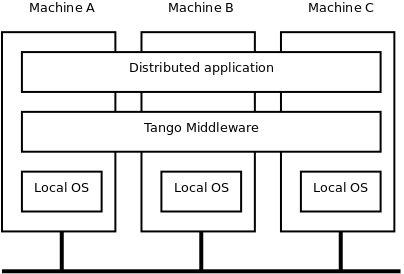
\includegraphics[width=0.5\textwidth]{imgs/TanenbaumDistributedSystemOrganization.png}
  \caption{From \cite{TanenbaumDistr}, A distributed system organized as middleware} \label{fig:TanenbaumDistributedSystemOrganization}}
  \end{figure}

  \begin{table}
  \centering{
   \begin{tabular}{|l|l|}
    \hline
    Access & Hide differences in data representation and how a resource is accessed \\ \hline
    Location & Hide where a resource is located \\ \hline
    Migration & Hide that a resource may move to another location \\ \hline
    Relocation & Hide that a resource may be moved to another location while in use \\ \hline
    Replication & Hide that a resource is replicated \\ \hline
    Concurrency & Hide that a resource may be shared by several competitive users \\ \hline
    Failure & Hide a faulure and recovery of a resource \\ \hline
    Persistence & Hide whether a (software) resource is in memory or on disk \\ \hline
   \end{tabular}
   \caption{Distributed systems transparencies \label{tab:transparencies}}}
  \end{table}
\begin{itemize}
 \item Security threads, policies and mechanisms. Section \ref{sec:scenarios}. Go further that the Locking/Access control
 \item Why to secure it? Trust in a peripheral firewalls is not enough. Often communications between tango installations (different tango-db) requires firewall rules to allow it, but this doesn't allow to filter by agent or by who is allowed to access the information. In practice, what is filtered is an specific computer traffic, but this breaks many of the distributed system transparencies.\\ The example of the Beamlines (read) access to (a few but crucial) accelerator information is a great example of what means a security thread.\\The industrial example of ``do it fast'' or ``finish it now'' more often than thought hides an insecure system or even worst a ``bugged'' system. 
  \\
 \item Following the 3 layers structure of a distributed system \cite{TanenbaumDistr} to identify scenarios in section \ref{sec:scenarios} and solutions in sections \ref{sec:intercom}:
 \begin{itemize}
 \item Agent authentication in the presentation layer (section \ref{sec:presentationLayer}). Possible solutions as the zero-knowledge proof (section \ref{sec:auth}) and Secret Sharing (section \ref{sec:secretSharing}).
 \item Domain layer communications protection in section \ref{sec:domainLayer}. Trusted computing with elliptic curves \ref{sec:ecpk}, data communication with symmetric encryption in section \ref{sec:gRijndael} and stream cyphering in section \ref{sec:kdfStreaming})
 \item Ensure Data layer (section \ref{sec:dataLayer}) with homomorphic encryption (section \ref{sec:Homorph}) in the database.
 \end{itemize}
 \item The price of the information and the balance between the cost to ensure and the value of the ensured goods. Section \ref{sec:secLevel}
 \item Alert on possible attacks to protect against what is already saw as a security thread, section \ref{sec:attacks}, distinguishing between passive (section \ref{sec:passiveAttacks}), active (section \ref{sec:activeAttacks}) and side channels (section \ref{sec:sideChannelAttacks})
 \item Any already saw thread should have it countermeasure (section \ref{sec:countermeasures}) with special interest in intrusion detection (section \ref{sec:intrusionDetection})
 \item Final conclusions about ensuring protocols (section \ref{sec:protocols}) and IT environmental security (section \ref{sec:environment})
\end{itemize}

%%%%%
%
\section{Identifying scenarios \label{sec:scenarios}}

\begin{itemize}
 \item From the view from \cite{TanenbaumDistr} over the distributed system transparencies, what is implemented in \tango\, and what is not? Is any of the ``nots'' necessary to ensure a quality service.
 \item Confidentiality (encryption and authentication): information must be disclosed only \emph{to} the authorized and only \emph{by} the authorized),
 \item Integrity (authorization): only authorized can set in the system. That is, only who is authorized can change an attribute, send a command or store a property.
 \item Auditory: trace who access where (extremely useful for a security breach analysis).
 \item In terms of security threads, which is more representative from \cite{SecEngRossAnderson} for the current use case? Three may types: \emph{Hospital}, \emph{Bank}, \emph{Military Base} (from where the security threads usually comes from). Practical paranoia \cite{PractCryptoSchneier}
 \item Cryptosystem configuration, security levels and information classification. Section \ref{sec:secLevel}. Can be saw as the nowadays number of rotors from the times of the electro-mechanical machines of last century.
 \item Cryptosystem setup reset.
 \item Setup \& Public-Key distribution protocols \cite{SecEngRossAnderson} sec.3.7.2
 \item Secret Shared schemas for (k,n)-to decrypt or (k,n)-signants. Section \ref{sec:secretSharing}.
 \item multicast and events (\zmq) can be scenarios of secret splitting. Section \ref{sec:secretSharing}.
 \item 
 \item 
\end{itemize}

%%%%%
%
\subsection{Ensuring presentation layer \label{sec:presentationLayer}}

\begin{itemize}
 \item Agent authentication in a distributed system
 \item Ensuring communication between agents and between those agents with the user interfaces.
 \begin{itemize}
  \item \emph{Command}, \emph{Attribute}, \emph{Properties}: Authenticate who can do the \emph{read} and \emph{write} operations. Encrypted logging who did any change, with levels to grant access levelling.
  \item This can be compared with \emph{RFID} communication between card and readers, but adding communication in between the agents
 \end{itemize}
 \item Deal with multicast can event subscription and emission.
 \item 
 \item 
\end{itemize}

%%%%%
%
\subsection{Ensuring domain layer \label{sec:domainLayer}}

\begin{itemize}
 \item Trusted Computing and Hardware protections
 \item Ensure logging system
 \item 
\end{itemize}

%%%%%
%
\subsection{Ensuring data layer \label{sec:dataLayer}}

\begin{itemize}
 \item \tango\, database access control
 \item Ensuring between instrumentation and the agents out of the scope of this paper. This is a very dependant on the instrumentation manufacturers. From the iso layer level view, even if the access to the hardware is not networked, the agent communication to the instrumentation is \emph{data link layer} and this paper is focus in \emph{transport} and above layers.
 \item Homomorphic Encryption for Database access
 \item  
 \item 
\end{itemize}

%%%%%
%
\section{Security levels \label{sec:secLevel}}

\begin{itemize}
 \item Security levels: Open or unclassified, confidential, Secret, Top Secret.
 \item remember the German standard on this levelling and the European commission ``\emph{fiche 17}'' (``Exchange of EU classified information'')
\end{itemize}

%%%%%
%
\section{Communication hybrid schema \label{sec:intercom}}

\begin{itemize}
 \item Embedded in instrumentation, limited calculation capacity (it must behave indistinguishable if it's a huge server or an embedded board), limited bandwidth (Don't increase the current needs significantly): \emph{very good candidate for elliptic curves (section \ref{sec:ecpk}), generalized Rijndael (section \ref{sec:gRijndael}) and stream cipher (section \ref{sec:kdfStreaming})}.
 \item Public-key to agreed a season key as the usual hybrid systems. This session keys shall be used for symmetric or stream cyphering.
 \item Session keys refresh.
 \item Use the Symmetric key to seed a shared PseudoRandomGenerator as a key for a stream cipher of transmitted data and listened data between talkers
 \item \emph{PseudoRandomGenerator} (PRG), can be use the KeyDerivationFunction (KDF) of the Rijndael or better other possible alternatives
 \item 
 \item 
\end{itemize}

%%%%%
%
\subsection{Zero-knowledge proof for authentication \label{sec:auth}}
\begin{itemize}
 \item The agents in the distributed system must be authenticated to be sure that they hasn't been supplanted
 \item 
 \item 
\end{itemize}

%%%%%
%
\subsection{Secret Sharing and secret splitting \label{sec:secretSharing}}
\begin{itemize}
 \item Multicast and event system. When a event is emitted, many would be subscribed, but encryption must be only made once.
 \item To allow some one access to some specific data, perhaps it can require the ``grant'' from more than one agent of the distributed system. That is, to give it the key may (k,n) must act to.
 \item Authorization units may be bigger than one agent. A (k,n)-signature to have only one to verify for all.
\end{itemize}

%%%%%
%
\subsection{Elliptic curves for public key \label{sec:ecpk}}

\begin{itemize}
 \item Set institution set of curves with different sizes for different level of secrecy (or even different curves for a separable sets in the same secrecy level). Isogeny volcanoes \cite{secRickShareECs}.
 \item Capability to reset a curve setup on any of those secrecy levels (section \ref{sec:secLevel})
 \item 
 \item 
\end{itemize}

%%%%%
%
\subsection{Rijndael generalization for symmetric key \label{sec:gRijndael}}

\begin{itemize}
 \item How to decide the good parameters of Rijndael? (\#rounds,\#rows,\#columns,wordsize of the block and the key) \cite{gRijndael}
 \item Current AES has advantage on 32bit processor implementation, what about 64bits
 \item AESWrap \cite{rfc3394}
 \item Secrecy levels (section \ref{sec:secLevel})
 \item 
\end{itemize}

%%%%%
%
\subsection{Key Derivation Functions for stream ciphering \label{sec:kdfStreaming}}

\begin{itemize}
 \item 
 \item 
\end{itemize}

%%%%%
%
\subsection{Homomorphic Encryption \label{sec:Homorph}}
\begin{itemize}
 \item 
 \item 
\end{itemize}
<
%%%%%
%
\section{Brainstorming attacks \label{sec:attacks}}

\begin{itemize}
 \item
 \item 
\end{itemize}

%%%%%
%
\subsection{Passive attacks \label{sec:passiveAttacks}}

\begin{itemize}
 \item Eavesdropping
 \item Noise to block an alarm transmission
 \item 
 \item 
\end{itemize}

%%%%%
%
\subsection{Active attacks \label{sec:activeAttacks}}

\begin{itemize}
 \item Men-in-the-middle (active attacks) between agents
 \item Interruption: Break the public face, web site or gui. Kill a vital agent.
 \item Modification/Fabrication: Supplant agents.
 \item 
 \item 
\end{itemize}

%%%%%
%
\subsection{Side channel attacks \label{sec:sideChannelAttacks}}

\begin{itemize}
 \item
 \item 
\end{itemize}

%%%%%
%
\section{Attacks countermeasures \label{sec:countermeasures}}

\begin{itemize}
 \item
 \item 
\end{itemize}

%%%%%
%
\subsection{Intrusion Detection \label{sec:intrusionDetection}}

\begin{itemize}
 \item Detection and recovery
 \item 
 \item 
\end{itemize}

%%%%%
%
\section{Conclusions \label{sec:conclusions}}

\begin{itemize}
 \item Al those fields mention on this paper requires a much further detailed paper each.
 \item 
\end{itemize}

%%%%%
%
\subsection{Protocols \label{sec:protocols}}

\begin{itemize}
 \item Protocol layers \cite{Schneier:1995:ACP:572932}
 \item Security architecture patterns
 \item Trust ring vs. trust tree (institution CA until the leaves)
 \item Streaming protection systems (specially for DevEncoded transmission of big images when fast acquisitions)
 \item 
 \item 
\end{itemize}

%%%%%
%
\subsection{Environmental IT Security \label{sec:environment}}

\begin{itemize}
 \item The weakest brick: secure the transmission but store in a plain file system
 \item Human behaviour and psychology.
 \item 
 \item 
\end{itemize}

%%%%%
%
\subsection{Further work \label{sec:further}}

\begin{itemize}
\item \atk/ \taurus\, user authentication using PAM system (or equivalent in non unix-like systems). Any other user interface that can access tango.
\item in all the algorithms on this paper this must be taken into account to minimize redesigns.
\end{itemize}


\bibliographystyle{ieeetr}
\bibliography{../bibtex/sblanch.bib,../bibtex/standards.bib,../bibtex/ecc.bib,../bibtex/isogeny.bib,../bibtex/books.bib,../bibtex/crypto.bib,../bibtex/rfc.bib}

\end{document}
